\section{Details on Interpolation and Extrapolation} \label{appendix:methodology}

\subsection{Identifying Treatment Effects}
\label{app:method_identify}

\noindent In the main paper, we discuss three cases of attrition. Below, we elaborate on the methodology we use for each case. \\

\subsubsection{Fully Observed Outcomes}
\label{app:method_fullobs}

\noindent  In the case where we fully observe outcomes, we only need to address the compromised randomization
of treatment status in our empirical estimates (see Section \ref{section:methodology}). \\

\noindent Randomization into treatment and control for each cohort occurred after the cohort was split
into two subsamples balanced by gender, maternal IQ,
and number of siblings. Subjects from each subsample were then matched on HRI, and randomized
into their respective experimental groups. Sex, maternal IQ, number of siblings, and HRI
therefore comprise $Z$. Thus, to obtain an
unbiased estimate of the treatment effect, we regress the outcome variable on treatment status,
controlling for those four baseline variables, as well as for cohort. \\

\noindent We perform this estimation on 1,000 bootstrap resamples of the original ABC and CARE data. We take the
mean of the empirical bootstrap distribution as our point estimate, and the standard deviation
of the distribution as the standard error. We estimate these effects on the
pooled ABC and CARE sample, as well as the male and female subsamples. This allows us to generate
rates of return and benefit-cost ratios for the male subsample, the female subsample, and the pooled sample. \\
%Moreover, we are able to obtain more precise estimates of the treatment
%effect for males, as the data for females generally exhibit more noise. See Table \ref{table:nonipw} for the list of outcomes to which we apply this method.


\subsubsection{Partially Observed Outcomes}
\label{app:method_partialobs}

\noindent Given the small sample size of the ABC and CARE data, we consider outcome variables with fewer than 100 observations
to exhibit a sizable rate of attrition. These variables include parental income at ages 2, 3, 4, 5, 9, 12,
and 15, for which we observe no more than 91 subjects at any given age; and the health survey at
age 34, for which we observe no more than 72 subjects. \\

\noindent We weight each subject by
his/her propensity to select into treatment and propensity to respond. We estimate the
former with a logit model for treatment status, controlling for baseline
variables used to determine randomization into treatment status: cohort,
maternal IQ, number of siblings, HRI, and sex (in the case of pooled estimates). \\

\noindent To estimate the propensity to respond, we similarly estimate a logit model of observing the outcome,
controlling for treatment status and three additional covariates. The additional covariates are
chosen amongst a set of variables likely to be correlated with non-response rates for the outcome variable.
This set of variables includes baseline characteristics determining randomization,
baseline variables other than randomization, and observed adult outcomes potentially affected by
treatment. To select these variables, we estimate the
aforementioned logit model controlling for treatment status and every three-variable combination from
the described set of variables. The model with the lowest Akaike Information Criteria (AIC) value is used to estimate the propensity
to respond. We limit the number of covariates in our logit models to three as this noticeably reduces the frequency of bootstrap resamples which exhibit perfect separation in the covariates. \\

\noindent To estimate the treatment effect, we regress the outcome of interest on treatment status, and weight the
observations by the inverse of the product of the two propensity scores estimated with the method
documented in Section~\ref{section:methodology} in the main paper. This procedure is performed on 1,000 bootstrap resamples of the original ABC and CARE data.
We take the mean of the empirical bootstrap distribution as our point estimate, and the standard deviation
of the distribution as the standard error. Again, we carry out this procedure for the
pooled sample, male subsample, and female subsample. \\

\paragraph{Parental Income}

\noindent Parental income is reported at ages 0, 2, 3, 4, 5, 9, 12, and 15, allowing us to directly estimate
the treatment effect on parental income at those ages. Given the rate of attrition in
parental income from age 2 onwards, we estimate these treatment effects accounting for attrition
with IPW weights.
To obtain a more complete picture of how the
program affected parental income, we estimate the treatment effect in the missing ages by linearly
interpolating the treatment effects between the years for which we observe parental income. We assume
there are no impacts from age 16 onwards (i.e. a treatment effect of 0). \\


\subsubsection{Fully Missing Outcomes}
\label{app:method_noobs}

\paragraph{Subject Income}

\noindent Labor and public-transfer income of subjects are observed intermittently at ages 21 and 30 only. In order
to obtain a complete measure of the impact of the ABC and CARE programs on subject income, we interpolate
the income streams of subjects for ages 22 to 29, and extrapolate income streams for ages
31 to 67 using three auxiliary datasets: NLSY79, CNLSY, and PSID. \\

\noindent We assume common support between the auxiliary
datasets and the analysis sample. This is required in order for us to reliably use external data to provide inference for the ABC and CARE samples. Figure~\ref{fig:support} validates this
assumption by displaying the overlapping support sets of ABC and CARE and our auxiliary data for
the variables used to interpolate and extrapolate earnings. For details about these datasets, see Appendix \ref{app:subject_income}. \\


\begin{figure}[H]
	\caption{Support of ABC and Auxiliary Data} \label{fig:support}
	\begin{subfigure}[h]{0.8\textwidth}
	\centering
	\caption{Income at Age 21} \label{fig:support_inc21}
	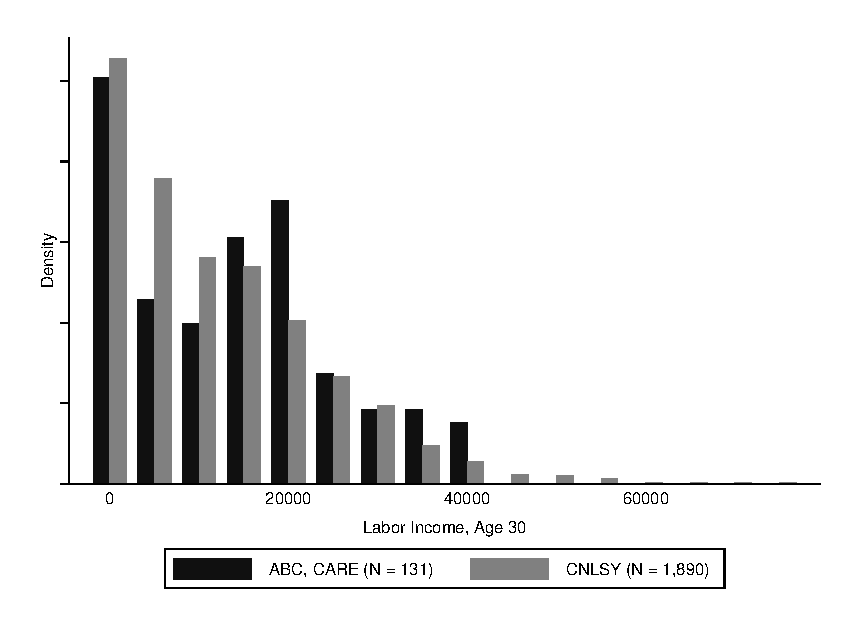
\includegraphics[width=\textwidth]{AppOutput/Methodology/support_inc21.eps}
	\end{subfigure}
	
	\begin{subfigure}[h]{0.8\textwidth}
	\centering
	\caption{Income at Age 30} \label{fig:support_inc30}
	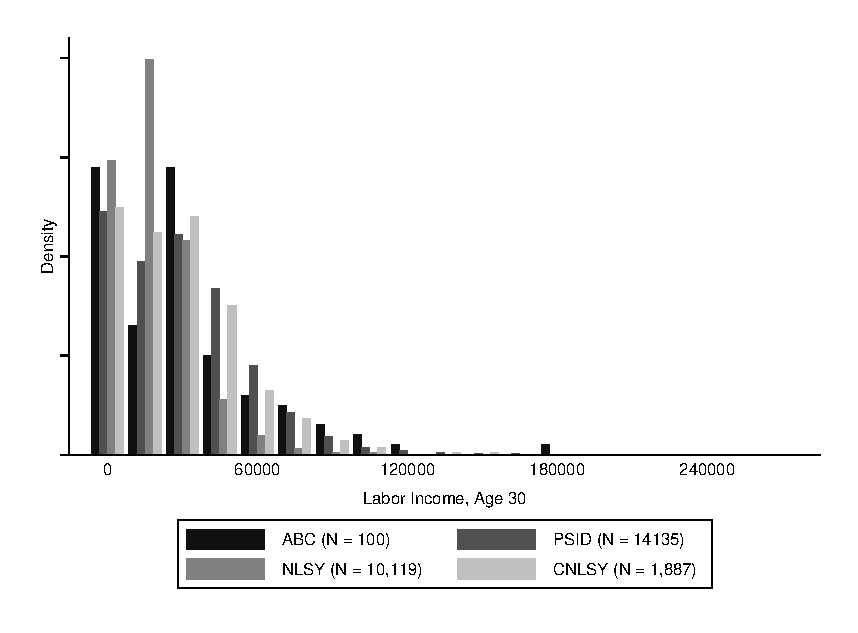
\includegraphics[width=\textwidth]{AppOutput/Methodology/support_inc30.eps}
	\end{subfigure}
\end{figure}




\begin{figure}[H]
	\ContinuedFloat
	\begin{subfigure}[h]{0.8\textwidth}
	\centering
	\caption{Subject's Years of Education} \label{fig:support_educ}
	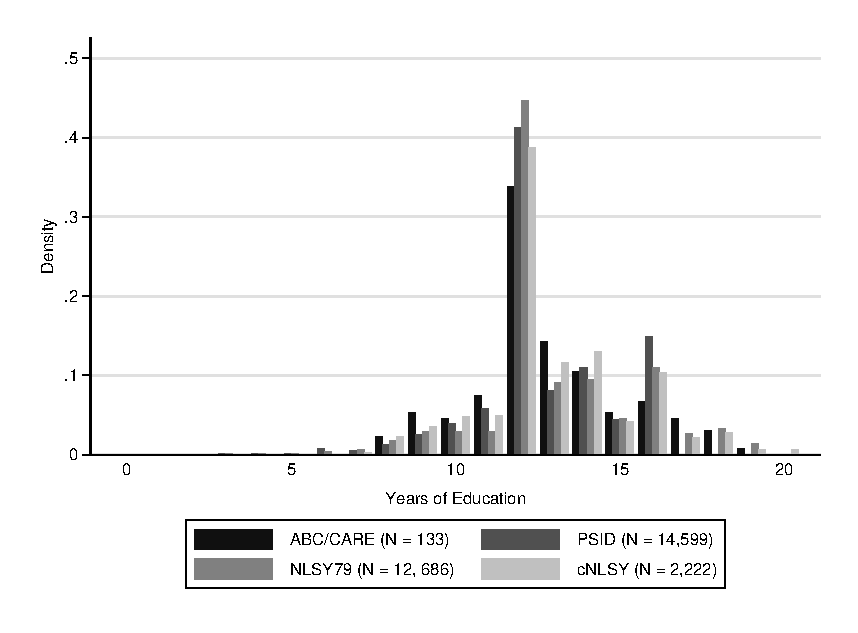
\includegraphics[width=\textwidth]{AppOutput/Methodology/support_educ.eps}
	\end{subfigure}
	
	\begin{subfigure}[h]{0.8\textwidth}
	\centering
	\caption{Mother's Years of Education} \label{fig:support_meduc}
	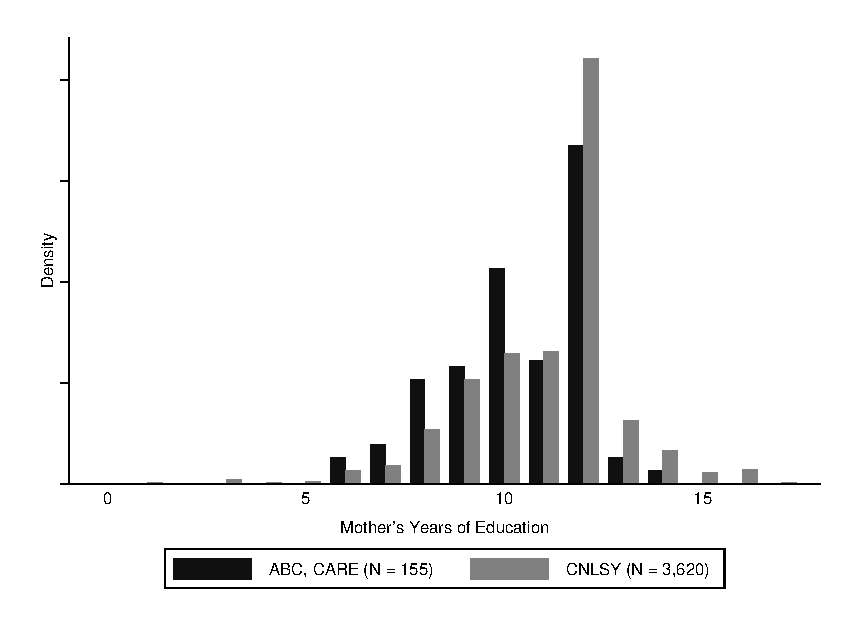
\includegraphics[width=\textwidth]{AppOutput/Methodology/support_momed.eps}
	\end{subfigure}
	
\end{figure}
	
\begin{figure}[H]
	\ContinuedFloat
	\begin{subfigure}[h]{0.8\textwidth}
	\centering
	\caption{Average PIAT Math Scores, Ages 5--7} \label{fig:support_math}
	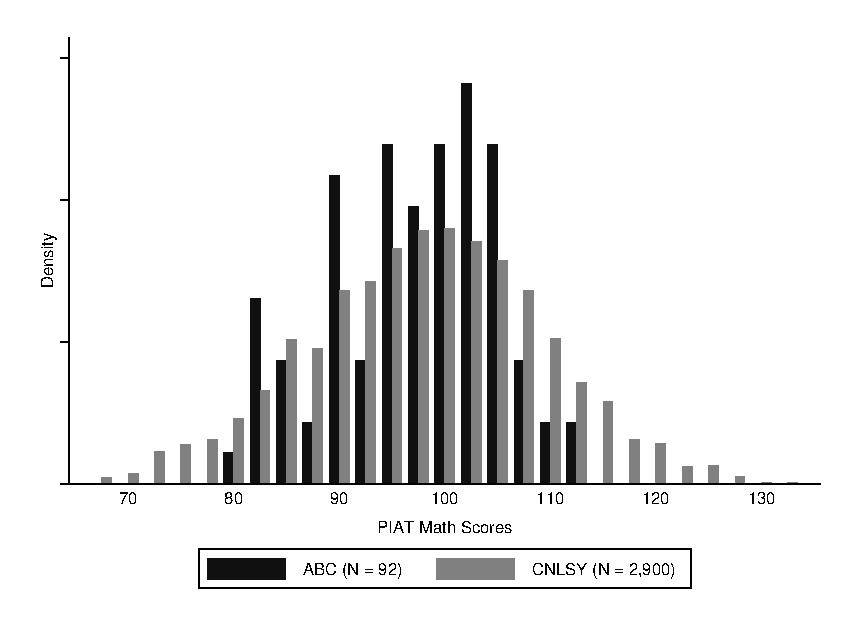
\includegraphics[width=\textwidth]{AppOutput/Methodology/support_math.eps}
	\end{subfigure}
	
	\begin{subfigure}[h]{0.8\textwidth}
	\centering
	\caption{Body Mass Index, Age 34} \label{fig:support_bmi}
	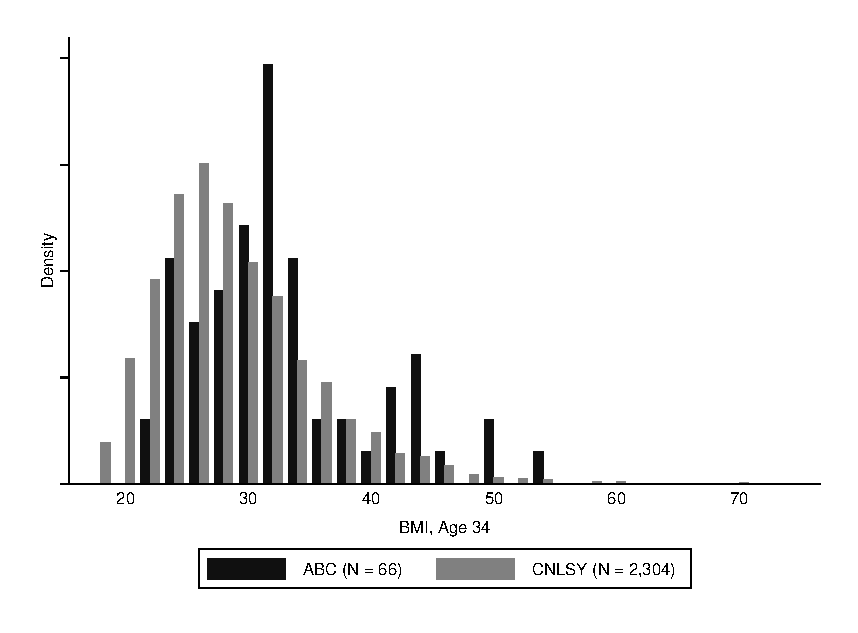
\includegraphics[width=\textwidth]{AppOutput/Methodology/support_bmi.eps}
	\end{subfigure}
	
	\floatfoot{
	\noindent Note: These graphs display the support of ABC, PSID, NLSY, and CNLSY
	for variables we use to project future earnings. PIAT math
	scores are averaged over ages 5--7.
	}
\end{figure}


\noindent Both labor and public-transfer income are interpolated using the exact same methodology, so we restrict
our attention to interpolating labor income. We employ the CNLSY dataset to model labor
income at each age from 22 to 29. We use ordinary least squares and regress labor income of
CNLSY subjects on background characteristics and early adult outcomes. Variables for background
characteristics consist of an indicator for being  black, mother's education, and sex. Variables
used to interpolate early adult outcomes consist of labor income at ages 21 and 30, years of education at age 30, average
PIAT math scores from ages 5 to 10, and BMI at age 34. We estimate the model on 1,000 bootstrap
resamples of the CNLSY to obtain a measure of prediction error, and denote the vectors of coefficients
\emph{for the outcome variables} by $\beta_{a,s}$, where $a \in \{22, 23, \dots, 29\}$ denotes age, and
$s \in \{1,2,\dots,1,000\}$ indexes the bootstrap samples. \\

% We impose two restrictions on the CNLSY dataset: one on birth year, and one on income.
% In regard to birth year, we limit the sample to subjects born in between 1978 and 1983. As our
% CNLSY data extends up to 2012, this implies that we use the most recent data from the CNLSY
% where individuals are of age 29 to 34.

% Given the biennial nature of the CNLSY, we observe each subject at either the odd ages or even
% ages. Not only will this reduce the size of our sample on which we fit our prediction model
% at each age, but possibly introduce biases associated with the odd-aged and even-aged cohorts.
% To address this issue, we perform a linear interpolation on the variables in the CNLSY data
% that enter into our prediction model. This allows us to estimate our prediction model on
% all subjects of the CNLSY satisfying our restrictions at every age.

% We further restrict the CNLSY sample to individuals with labor income fewer than
% \$300,000 (USD 2014) at any given year. With the mean labor income in the ABC
% sample being \$12,232.43 at age 21 and \$32,781.96 at age 30 (USD 2014), and the maximum reported
% being \$189,937.50, the cut-off we impose on the auxiliary data is high enough
% so that everyone in the ABC sample is represented, yet low enough to
% exclude high-earning individuals in the auxiliary sample that do not reflect the ABC sample well.

\noindent The outcome variables we use as independent variables to fit the model to the CNLSY data are also
observed in the ABC and CARE data, and we are able to calculate the treatment effects on each of these outcomes
using the procedures described in Appendix \ref{app:method_fullobs} and Appendix \ref{app:method_partialobs}. We
obtain these estimates for 1,000 bootstrap resamples of both the ABC and CARE data, and denote the vectors of
coefficients by $\gamma_r$, where $r \in \{1,2,\dots,1,000\}$ indexes the bootstrap samples. \\

\noindent To interpolate the treatment effect on subject labor income at age $a$, we take the dot product
of $\beta_{a, s}$ and $\gamma_r$ for all $s,r$ pairs, resulting in 1,000,000 scalars. We reintroduce
prediction error by first randomly drawing residuals from our fitted model on the auxiliary data and assigning
them to the ABC and CARE subjects. We then take the mean difference of these residuals across treatment and control
groups, and add it to the previously described scalar. We do this for all 1,000,000 scalars. These scalars form the empirical
bootstrap distribution of the treatment effect. Note that
we bypass the estimation of the subjects' actual incomes, of which we are unable to obtain an
unbiased estimate. Instead, we directly obtain an unbiased estimate of the treatment effect. This
method implies that the impacts of the treatment on adult labor income can be expressed through
the observed early-adult outcomes. In this case, the observed early-adult outcomes are labor income at ages 21 and
30, years of education at age 30, average PIAT math scores from ages 5 to 10, and BMI at age 34. Since $\gamma_r$ has
been adjusted to address selection into treatment and attrition in the ABC and CARE data, the bootstrap distribution
is devoid of selection and attrition issues. In addition, the bootstrap distribution captures
the error stemming from the ABC and CARE datasets, and prediction error of the model fitted to the CNLSY dataset.
We take the mean of the empirical bootstrap distribution as our point estimate, and the standard deviation
of the distribution as the standard error. Again, we carry out this procedure for the
pooled, male, and female samples. \\

\noindent To extrapolate labor income, we employ the NLSY79 and PSID datasets. We execute the same estimation
strategy as above, but with a reduced set of control variables in order to limit the number
of dropped cases. Specifically, the set of background variables we control for include an indicator for
being black and gender of the subject. As the NLSY79 and PSID are not as rich as the CNLSY, we also
restrict our outcome variables to years of education at age 30 and subject labor income at age 30. \\
% Similar to the CNLSY, we restrict the PSID to individuals born between 1945 and 1980. As the PSID
% extends until 2013, this means we are using the most recent subsample of individuals aged 30 to 67.
% We do not impose a restriction on birth year on the NLSY as all respondents are aged between 47 and 55
% at the time of the last interview (conducted in 2012). For both the PSID and NLSY, subjects with labor
% income exceeding \$300,000 (USD 2014) are again excluded. Like the CNLSY, because of the biennial
% nature of the PSID and NLSY, we apply a linear interpolation to both data sets.

\noindent We estimate the vectors $\beta_{a, s}$ for $a \in \{31, 32, \dots, 67\}$ and $\gamma_r$, where
$s,r \in \{1,2,\dots,1,000\}$ index the bootstrap samples, and take the dot product of every pair of
$\beta_{a,s}$ and $\gamma_r$ vectors to obtain the empirical bootstrap distribution of the treatment
effect on labor income past age 30. We take the mean of the distribution to be the point estimate,
and the standard deviation of the distribution to be the standard error. \\

%The same procedure is carried out to interpolate and extrapolate transfer income, where we instead
%utilize transfer income as the dependent variable in the regressions on our auxiliary datasets.

\noindent The same procedure is carried out to interpolate public-transfer income, where we instead utilize public-transfer
income as the dependent variable in the regressions on our auxiliary datasets. In the case of
extrapolating public-transfer income from welfare, unemployment benefits, AFDC, and food stamps, we also apply
the same methodology as for labor income. However, in the case of disability insurance, social
security, and supplemental security income, we apply an alternative approach. For these cases, we estimate
the probability each ABC and CARE individual claims each of those benefits at ages 31--67, and multiply those
probabilities by the average annual claims of each type of public transfer reported by the Social
Security Administration in 2014. See Appendix \ref{section:FAM_ABC_impute}
for an explanation of how we estimate these probabilities. For each age, we sum across our estimates of
each type of public transfer received to obtain the total public-transfer income of ABC subjects. \\


\paragraph{Health Costs}

\noindent We predict health care costs from age 30 up to age 79, and criminal costs from birth
up to age 50. We then evaluate the predicted outcomes as if observed, and estimate the
treatment effect on those data.\\

\noindent As health outcomes are simulated using a set of variables exhibiting a high rate of attrition, the
predicted health outcomes exhibit an equal rate of attrition. We therefore employ the method described
in Appendix \ref{app:method_partialobs} to estimate the treatment effect on health care costs at
every age from 30 through 79, conditional on survival up to each age. \\

\paragraph{Crime Costs}

\noindent In the case of crime costs, we are able to predict costs for more than 100 individuals in the
sample. We therefore utilize the method described in subsection \ref{app:method_fullobs}
to estimate the treatment effect on the cost of criminal activity at every age from birth until age 50. \\


\begin{table}[H]
\begin{threeparttable}
\caption{Variables Estimated without IPW}
\label{table:nonipw}
\centering
% CONTENT CREATED ON SPREADSHEET, TREAT AS A .CSV (TAB DELIMITED)
% CAN BE COPIED INTO A SPREADSHEET PROGRAM (EXCEL, LIBRECALC) FOR EDITING
\begin{tabular}{l l}
\toprule
Variable	&	Age	\\
\midrule			
IQ Standard Score	&	2, 3, 4, 5, 6, 7, 8, 12, 15, 21	\\
PIAT Math Standard Score	&	7	\\
Home Total Score	&	0.5, 1.5, 2.5, 3.5, 4.5, 8	\\
Mother Works	&	2, 3, 4, 5	\\
Biological Mother's Education Level	&	2, 3, 4, 5, 9	\\
Father is Home	&	2, 3, 4, 5	\\
Ever Adopted	&		NA \\
Graduated High School	&	NA	\\
Attended Vocation/Tech/Community College	&	NA	\\
Earned Degree from 4-year College	&	NA	\\
Years of Education	&	30	\\
Works a Job	&	30	\\
Total Felony Arrests	&	Mid-30s	\\
Total Misdemeanor Arrests	&	Mid-30s	\\
Total Years Incarcerated	&	30	\\
Self-reported Health	&	30	\\
Number of Cigarettes Smoked Per Day Last Month	&	30	\\
Number of Days Drank Alcohol Last Month	&	30	\\
Number of Days Binge Drank Alcohol Last Month	&	30	\\
Program Costs	&	0--26	\\
Control Contamination Costs	&	0--26	\\
Education Costs	&	0--26	\\
Medical Expenditure &	8--30	\\
Justice System Costs	&	0--50	\\
Prison Costs	&	0--50	\\
Victimization Costs	&	0--50	\\
\bottomrule			
\end{tabular}
\begin{tablenotes}
\footnotesize
\item Note: The table above lists the variables for which we do not apply IPW when estimating
treatment effects.
\end{tablenotes}
\end{threeparttable}
\end{table}



\begin{sidewaystable}[H]
\caption{Model Selection for Attrition IPW \\ Pooled }
\label{table:ms_attrit_pooled}
\centering
\begin{adjustbox}{max width=\textwidth}
\begin{threeparttable}
% CONTENT CREATED ON SPREADSHEET, TREAT AS A .CSV (TAB DELIMITED)
% CAN BE COPIED INTO A SPREADSHEET PROGRAM (EXCEL, LIBRECALC) FOR EDITING
\scriptsize
\begin{tabular}{l r r l l l}
\toprule											
Partially Observed Outcomes	&	Age	&	N	&	\multicolumn{3}{c}{Variables Used to Produce IPW}	\\
\midrule	
IQ Score 				& 6.5 	& 126   & High Risk Index (HRI)	& APGAR 1 min.	&  Cohort \\
IQ Score 				& 7 	& 118   & High Risk Index (HRI)	& APGAR 5 min.	&  Cohort \\
IQ Score 				& 8 	& 125   & High Risk Index (HRI)	& APGAR 1 min.	&  Cohort \\
\\										
Achievement Score 		& 5.5	& 105 	& High Risk Index (HRI)	& APGAR 1 min.	&  Cohort \\ 
Achievement Score 		& 6		& 124 	& High Risk Index (HRI)	& APGAR 1 min.	&  Cohort \\ 
Achievement Score 		& 6.5	& 89 	& High Risk Index (HRI)	& APGAR 1 min.	&  Cohort \\ 
Achievement Score 		& 7		& 90 	& High Risk Index (HRI)	& APGAR 1 min.	&  Cohort \\ 
Achievement Score 		& 7.5	& 121 	& High Risk Index (HRI)	& APGAR 1 min.	&  Cohort \\ 
Achievement Score 		& 8		& 123 	& High Risk Index (HRI)	& APGAR 1 min.	&  Cohort \\ 
Achievement Score 		& 8.5	& 122 	& High Risk Index (HRI)	& APGAR 5 min.	&  Cohort \\ 
\\
Parental Labor Income	&	1.5	&	112	& Mother's Age at Baseline	& APGAR 1 min.	&  Cohort \\
 Parental Labor Income	&	2.5	&	112	&	Mother's Age at Baseline	& APGAR 1 min.	&  Cohort \\
 Parental Labor Income	&	3.5	&	110	&	Mother's Age at Baseline	& APGAR 1 min.	&  Cohort \\
 Parental Labor Income	&	8	&	87	&	High Risk Index (HRI)	& APGAR 1 min.	&  Cohort \\
 Parental Labor Income	&	12	&	108	&	High Risk Index (HRI)	& APGAR 1 min.	&  Cohort \\
 Parental Labor Income	&	15	&	92	&	APGAR 5 min. & 	Premature at Birth & Number of Siblings, Baseline \\
 Parental Labor Income	&	21	&	73	&	High Risk Index (HRI)	& APGAR 1 min.	&  Cohort \\
\\
HOME Score				& 8		& 	100 & 	High Risk Index (HRI)	& APGAR 1 min.	&  Cohort \\
\\
Father at Home			& 8		& 	116 & 	High Risk Index (HRI)	& APGAR 1 min.	&  Cohort \\
\\
Subject Public Transfer Income	&	21	&	105	& High Risk Index (HRI) & APGAR 1 min. & Cohort \\
 \\
Total Felony Arrests		& Mid-30s	& 115 &	APGAR 1 min. & APGAR 5 min. & Cohort	\\
Total Misdemeanor Arrests	& Mid-30s	& 115 &	APGAR 1 min. & APGAR 5 min. & Cohort	\\
 \\
 Self-reported Health	&	Mid-30s	&	92	&	APGAR 1 min. & APGAR 5 min. & Premature at Birth	\\
 Self-reported Drug User	&	Mid-30s	&	89	&	APGAR 1 min. & APGAR 5 min. & Premature at Birth	\\
 Systolic Blood Pressure (mm Hg)	&	Mid-30s	&	90	&	APGAR 1 min. & Premature at Birth & Number of Siblings, Baseline	\\
 Diastolic Blood Pressure (mm Hg)	&	Mid-30s	 &	90	&	APGAR 1 min. & Premature at Birth & Number of Siblings, Baseline	\\
 Prehypertension, Sys. B.P. $>$ 120 or Dys. B.P. $>$ 80	&	Mid-30s	&	90	&	APGAR 1 min. & Premature at Birth & Number of Siblings, Baseline	\\
 Hypertension, Sys. B.P. $>$ 140 or Dys. B.P. $>$ 90	&	Mid-30s	&	90	&	APGAR 1 min. & Premature at Birth & Number of Siblings, Baseline	\\
 High-Density Lipoprotein (HDL) Cholesterol (mg/dL)	&	Mid-30s	&	93	&	APGAR 1 min. & Premature at Birth & Number of Siblings, Baseline	\\
 Dyslipidemia (HDL $<$ 40 mg/dL)	&	Mid-30s	&	93	&	APGAR 1 min. & Premature at Birth & Number of Siblings, Baseline	\\
 Hemoglobin Level (\%)	&	Mid-30s	&	92	&	APGAR 1 min. & Premature at Birth & Number of Siblings, Baseline	\\
 Prediabetes, Hemoglobin $>$ 5.7\%	&	Mid-30s	&	92	&	APGAR 1 min. & Premature at Birth & Number of Siblings, Baseline	\\
 Diabetes, Hemoglobin $>$ 6.5\%	&	Mid-30s	&	92	&	APGAR 1 min. & Premature at Birth & Number of Siblings, Baseline	\\
 Vitamin D Deficiency ($<$ 20 ng/mL)	&	Mid-30s	&	93	&	APGAR 1 min. & Premature at Birth & Number of Siblings, Baseline	\\
 Measured BMI	&	Mid-30s	&	88	&	APGAR 1 min. & APGAR 5 min. & Premature at Birth \\
 Obesity (BMI $>$ 30)	&	Mid-30s	&	90	&	APGAR 1 min. & APGAR 5 min. & Premature at Birth \\
 Severe Obesity (BMI $>$ 35)	&	Mid-30s	&	91	&	APGAR 1 min. & APGAR 5 min. & Premature at Birth \\
 Waist-hip Ratio	&	Mid-30s	&	84	& APGAR 1 min. & Premature at Birth & Number of Siblings, Baseline \\
 Abdominal Obesity	&	Mid-30s	&	84	& APGAR 1 min. & Premature at Birth & Number of Siblings, Baseline \\
 Framingham Risk Score	&	Mid-30s	&	88	& APGAR 1 min. & Premature at Birth & Number of Siblings, Baseline \\
 Brief Symptom Survey (BSI) Score & Mid-30s & 92 &	APGAR 1 min. & APGAR 5 min. & Premature at Birth	\\
\bottomrule											
\end{tabular}
\begin{tablenotes}
\tiny
\item Note: The table above lists the variables used to generate the component of the
inverse probability weights we use to account for attrition. To obtain this
component for attrition, we estimate a logit model for observing the outcome variable,
controlling for treatment, and three additional covariates depending on the outcome
variable. The additional variables are chosen from a list of covariates possibly affecting
response rates. The set yielding the lowest Akaike Information Criteria value is used to
generate the IPW weights, and are listed in the table above.
\end{tablenotes}
\end{threeparttable}
\end{adjustbox}
\end{sidewaystable}

\begin{sidewaystable}[H]
\caption{Model Selection for Attrition IPW \\ Females }
\label{table:ms_attrit_pooled}
\centering
\begin{adjustbox}{max width=\textwidth}
\begin{threeparttable}
% CONTENT CREATED ON SPREADSHEET, TREAT AS A .CSV (TAB DELIMITED)
% CAN BE COPIED INTO A SPREADSHEET PROGRAM (EXCEL, LIBRECALC) FOR EDITING
\tiny
\begin{tabular}{l r r l l l}
\toprule										
Variable	&	Age	&	Obs.	&	(1)	&	(2)	&	(3)	\\
\midrule											
Parental Labor Income	&	2	&	33	&	Subject Birth Year	&	Mother Works, age 5	&	Father works before pregnancy	\\
Parental Labor Income	&	3	&	33	&	Subject Birth Year	&	Mother Works, age 5	&	Father works before pregnancy	\\
Parental Labor Income	&	4	&	31	&	Subject Birth Year	&	Father works before pregnancy	&	Siblings in Household, age 5	\\
Parental Labor Income	&	5	&	44	&	Mother Works before Pregnant	&	Mother Works, age 5	&	Father works before pregnancy	\\
Parental Labor Income	&	9	&	40	&	Mother Works, age 5	&	HRI 2: No Maternal Relatives	&	Father works before pregnancy	\\
Parental Labor Income	&	12	&	45	&	Subject Birth Year	&	Mother Works, age 5	&	Father works before pregnancy	\\
Parental Labor Income	&	15	&	47	&	Mother Works, age 5	&	HRI 2: No Maternal Relatives	&	Father works before pregnancy	\\
\\
Subject Labor Income	&	21	&	51	&	Mother's WAIS Performance IQ	&	Mother's Age at entry	&	ASR t-score: Attention Deficit and Hyperactivity	\\
Subject Labor Income	&	30	&	53	&	HRI 10: Other special circumstances	&	ASR t-score: Substance Abuse	&	Years of Education	\\
Subject Public Transfer Income	&	21	&	49	&	Mother's WAIS Comprehension	&	Number of cigarettes smoked per day	&	ASR t-score: Attention Deficit and Hyperactivity	\\
Subject Public Transfer Income	&	30	&	53	&	HRI 10: Other special circumstances	&	ASR t-score: Substance Abuse	&	Years of Education	\\
\\
Self-reported Health	&	Mid-30s	&	40	&	Length at birth	&	ASR t-score: Substance Abuse	&	Years of Education	\\
Self-reported Drug User	&	Mid-30s	&	40	&	Length at birth	&	ASR t-score: Substance Abuse	&	Years of Education	\\
Systolic Blood Pressure (mm Hg)	&	Mid-30s	&	40	&	Length at birth	&	ASR t-score: Substance Abuse	&	Years of Education	\\
Diastolic Blood Pressure (mm Hg)	&	Mid-30s	&	40	&	Length at birth	&	ASR t-score: Substance Abuse	&	Years of Education	\\
Prehypertension, Sys. B.P. $>$ 120 or Dys. B.P. $>$ 80	&	Mid-30s	&	40	&	Length at birth	&	ASR t-score: Substance Abuse	&	Years of Education	\\
Hypertension, Sys. B.P. $>$ 140 or Dys. B.P. $>$ 90	&	Mid-30s	&	40	&	Length at birth	&	ASR t-score: Substance Abuse	&	Years of Education	\\
High-Density Lipoprotein (HDL) Cholesterol (mg/dL)	&	Mid-30s	&	40	&	Length at birth	&	ASR t-score: Substance Abuse	&	Years of Education	\\
Dyslipidemia (HDL $<$ 40 mg/dL)	&	Mid-30s	&	40	&	Length at birth	&	ASR t-score: Substance Abuse	&	Years of Education	\\
Hemoglobin Level (\%)	&	Mid-30s	&	39	&	Length at birth	&	ASR t-score: Substance Abuse	&	Years of Education	\\
Prediabetes, Hemoglobin $>$ 5.7\%	&	Mid-30s	&	39	&	Length at birth	&	ASR t-score: Substance Abuse	&	Years of Education	\\
Diabetes, Hemoglobin $>$ 6.5\%	&	Mid-30s	&	39	&	Length at birth	&	ASR t-score: Substance Abuse	&	Years of Education	\\
Vitamin D Deficiency ($<$ 20 ng/mL)	&	Mid-30s	&	40	&	Length at birth	&	ASR t-score: Substance Abuse	&	Years of Education	\\
Measured BMI	&	Mid-30s	&	40	&	Length at birth	&	ASR t-score: Substance Abuse	&	Years of Education	\\
Obesity (BMI $>$ 30)	&	Mid-30s	&	40	&	Length at birth	&	ASR t-score: Substance Abuse	&	Years of Education	\\
Severe Obesity (BMI $>$ 35)	&	Mid-30s	&	40	&	Length at birth	&	ASR t-score: Substance Abuse	&	Years of Education	\\
Waist-hip Ratio	&	Mid-30s	&	37	&	Length at birth	&	ASR t-score: Substance Abuse	&	Years of Education	\\
Abdominal Obesity	&	Mid-30s	&	37	&	Length at birth	&	ASR t-score: Substance Abuse	&	Years of Education	\\
Framingham Risk Score	&	Mid-30s	&	39	&	Length at birth	&	ASR t-score: Substance Abuse	&	Years of Education	\\
\bottomrule																																	
\end{tabular}
\begin{tablenotes}
\tiny
\item Note: The table above lists the variables used to generate the component of the
inverse probability weights we use to account for attrition. To obtain this
component for attrition, we estimate a logit model for observing the outcome variable,
controlling for treatment, and three additional covariates depending on the outcome
variable. The additional variables are chosen from a list of covariates possibly affecting
response rates. The set yielding the lowest Akaike Information Criteria value is used to
generate the IPW weights, and are listed in the table above.
\end{tablenotes}
\end{threeparttable}
\end{adjustbox}
\end{sidewaystable}



\begin{sidewaystable}[H]
\caption{Model Selection for Attrition IPW \\ Males }
\label{table:ms_attrit_pooled}
\centering
\begin{adjustbox}{max width=\textwidth}
\begin{threeparttable}
% CONTENT CREATED ON SPREADSHEET, TREAT AS A .CSV (TAB DELIMITED)
% CAN BE COPIED INTO A SPREADSHEET PROGRAM (EXCEL, LIBRECALC) FOR EDITING
\tiny
\begin{tabular}{l r r l l l}
\hline\hline											
Variable	&	Age	&	Obs.	&	(1)	&	(2)	&	(3)	\\
\hline											
Parent Labor Income	&	2	&	39	&	Subject Birth Year	&	Mother Works, age 3	&	Siblings in Household, age 3	\\
Parent Labor Income	&	3	&	39	&	Subject Birth Year	&	Mother Works, age 3	&	Father works before pregnancy	\\
Parent Labor Income	&	4	&	38	&	Subject Birth Year	&	Mother Works, age 4	&	Siblings in Household, age 3	\\
Parent Labor Income	&	5	&	42	&	Mother Works, age 3	&	Mother Works, age 4	&	Siblings in Household, age 5	\\
Parent Labor Income	&	9	&	42	&	Mother Works, age 3	&	Father home, age 5	&	Siblings in Household, age 5	\\
Parent Labor Income	&	12	&	46	&	Subject Birth Year	&	Mother Works, age 4	&	Father home, age 5	\\
Parent Labor Income	&	15	&	43	&	Mother Works, age 4	&	Father works before pregnancy	&	Siblings in Household, age 5	\\
\\
Subject Labor Income	&	21	&	45	&	HRI 10: Other special circumstances	&	Gestational Age $\leq$ 36	&	ASR t-score: Substance Abuse	\\
Subject Labor Income	&	30	&	47	&	Father's Age at entry	&	Mother Married at entry	&	ASR t-score: Substance Abuse	\\
Subject Public Transfer Income	&	21	&	48	&	Father's Age at entry	&	Gestational Age $\leq$ 36	&	Years of Education	\\
Subject Public Transfer Income	&	30	&	48	&	Mother's WAIS Performance IQ	&	ASR t-score: Antisocial Personality Problems	&	Had physical exam for illness in last 2 years	\\
\\
Self-reported Health	&	Mid-30s	&	30	&	HRI 2: No Maternal Relatives	&	ASR t-score: Substance Abuse	&	ASR t-score: Antisocial Personality Problems	\\
Self-reported Drug User	&	Mid-30s	&	27	&	Gestational Age $\leq$ 36	&	ASR t-score: Substance Abuse	&	Had physical exam for illness in last 2 years	\\
Systolic Blood Pressure (mm Hg)	&	Mid-30s	&	28	&	Gestational Age $\leq$ 36	&	ASR t-score: Substance Abuse	&	Had physical exam for illness in last 2 years	\\
Diastolic Blood Pressure (mm Hg)	&	Mid-30s	&	28	&	Gestational Age $\leq$ 36	&	ASR t-score: Substance Abuse	&	Had physical exam for illness in last 2 years	\\
Prehypertension, Sys. B.P. $>$ 120 or Dys. B.P. $>$ 80	&	Mid-30s	&	28	&	Gestational Age $\leq$ 36	&	ASR t-score: Substance Abuse	&	Had physical exam for illness in last 2 years	\\
Hypertension, Sys. B.P. $>$ 140 or Dys. B.P. $>$ 90	&	Mid-30s	&	28	&	Gestational Age $\leq$ 36	&	ASR t-score: Substance Abuse	&	Had physical exam for illness in last 2 years	\\
High-Density Lipoprotein (HDL) Cholesterol (mg/dL)	&	Mid-30s	&	31	&	Gestational Age $\leq$ 36	&	ASR t-score: Substance Abuse	&	Had physical exam for illness in last 2 years	\\
Dyslipidemia (HDL $<$ 40 mg/dL)	&	Mid-30s	&	31	&	Gestational Age $\leq$ 36	&	ASR t-score: Substance Abuse	&	Had physical exam for illness in last 2 years	\\
Hemoglobin Level (\%)	&	Mid-30s	&	31	&	Gestational Age $\leq$ 36	&	ASR t-score: Substance Abuse	&	Had physical exam for illness in last 2 years	\\
Prediabetes, Hemoglobin $>$ 5.7\%	&	Mid-30s	&	31	&	Gestational Age $\leq$ 36	&	ASR t-score: Substance Abuse	&	Had physical exam for illness in last 2 years	\\
Diabetes, Hemoglobin $>$ 6.5\%	&	Mid-30s	&	31	&	Gestational Age $\leq$ 36	&	ASR t-score: Substance Abuse	&	Had physical exam for illness in last 2 years	\\
Vitamin D Deficiency ($<$ 20 ng/mL)	&	Mid-30s	&	31	&	Gestational Age $\leq$ 36	&	ASR t-score: Substance Abuse	&	Had physical exam for illness in last 2 years	\\
Measured BMI	&	Mid-30s	&	26	&	Gestational Age $\leq$ 36	&	ASR t-score: Substance Abuse	&	Had physical exam for illness in last 2 years	\\
Obesity (BMI $>$ 30)	&	Mid-30s	&	28	&	Father works before pregnancy	&	ASR t-score: Substance Abuse	&	ASR t-score: Attention Deficit and Hyperactivity	\\
Severe Obesity (BMI $>$ 35)	&	Mid-30s	&	29	&	HRI 2: No Maternal Relatives	&	Mother's WAIS Comprehension	&	Number of times smoked marijuana	\\
Waist-hip Ratio	&	Mid-30s	&	25	&	Gestational Age $\leq$ 36	&	ASR t-score: Substance Abuse	&	Had physical exam for illness in last 2 years	\\
Abdominal Obesity	&	Mid-30s	&	25	&	Gestational Age $\leq$ 36	&	ASR t-score: Substance Abuse	&	Had physical exam for illness in last 2 years	\\
Framingham Risk Score	&	Mid-30s	&	27	&	Gestational Age $\leq$ 36	&	ASR t-score: Substance Abuse	&	Had physical exam for illness in last 2 years	\\
\hline\hline																							
\end{tabular}
\begin{tablenotes}
\tiny
\item Note: The table above lists the variables used to generate the component of the
inverse probability weights we use to account for attrition. To obtain this
component for attrition, we estimate a logit model for observing the outcome variable,
controlling for treatment, and three additional covariates depending on the outcome
variable. The additional variables are chosen from a list of covariates possibly affecting
response rates. The set yielding the lowest Akaike Information Criteria value is used to
generate the IPW weights, and are listed in the table above.
\end{tablenotes}
\end{threeparttable}
\end{adjustbox}
\end{sidewaystable}

\subsection{Internal Rate of Return}
\label{app:method_irr}

\noindent To estimate the internal rate of return, we must solve for $\rho$ in the equation below,

\begin{align}
\sum_{t=0}^T \frac{ \mathbb{E} (B_t - C_t)}{(1+\rho)^t} = 0,
\end{align}

\noindent where we let $T = 79$, define $B_t$ and $C_t$ to be the total benefits and costs of the
program at time $t$, and define $\mathbb{E}$ to be the sample mean. \\

\noindent All outcomes of the parents and subjects that we observe as having been affected by the program
are treated as benefits. For this to make sense, we reverse the sign of the monetized effect of the program
on specific outcomes. Costs of ABC and CARE consist only of the initial program costs from ages 0 to 5.
Table \ref{table:bc_comp} provides a full list of the benefits and costs of ABC and CARE. \\

\noindent We take the sum of the treatment effects on each component of the benefits to
be the total benefit, $B_t$, of the ABC and CARE programs (see Appendix \ref{app:method_identify} on how
we estimate these treatment effects). This includes parental income, subject labor income, and QALYs
(quality-adjusted life years).
Treatment effects on costs borne by the subject or society have their signs
reversed and are included as benefits. We do this for subject public-transfer income,
education costs, crime costs,
control contamination costs, and health costs. To account for deadweight loss, we
impose a marginal welfare cost of 50\% by multiplying public costs by a factor of
$1.5$.\footnote{There is no clear consensus on the marginal welfare cost of tax revenue. However,
most researchers estimate the welfare cost per tax dollar to be between \$0.30 and \$0.50. See
\citet{Feldstein_1999_REStat}, \citet{Heckman_Smith_1998_evaluating}, and \citet{Browning_1987_AER}.} Public costs include education costs up until age 17, jail costs, justice system costs, Medicare costs,
Medicaid costs, disability insurance claims, social security claims, and supplemental security
income. \\

\noindent Having constructed our cash flow, $\mathbb{E} (B_t - C_t)$, solving for $\rho$
reduces to an algebraic exercise. \\

\noindent As described in Appendix \ref{app:method_identify}, we estimate the treatment effect on each
component of the benefits and costs at time $t$ for the pooled, male, and
female samples. We do this for 1,000 bootstrap resamples of the original ABC and CARE data.
In the case of health costs and subject income, for which we employ auxiliary datasets to
estimate the treatment effects, we also obtain 1,000 bootstrap estimates from the auxiliary data
for every ABC and CARE bootstrap resample, resulting in a total of 1,000,000 estimates.
By reusing each bootstrap estimate of the treatment effect on outcomes that do not require any auxiliary data
set 1,000 times, we obtain a total of 1,000,000 estimates of the cash flow.
We estimate the IRR on each of those cash flows.
This is how we form our empirical bootstrap distribution of the IRR for the pooled, male, and female samples.
We take the mean of the distributions to be the point estimates, and we take the standard deviations
to be the standard errors. To construct the 80\% confidence intervals, we take the 10\textsuperscript{th}
and 90\textsuperscript{th} quantiles of each bootstrap distribution. \\

\begin{table}[H]
\begin{threeparttable}
\caption{Components of Benefits and Costs}
\label{table:bc_comp}
\centering
\begin{tabular}{l c c}
\toprule			
Variable & Sign Reversed	& Welfare Cost \\
	&		& Factor \\
\midrule
\textbf{Benefits} 	\\			
\quad Parent Income			& \\
\quad Subject QALY			& \\
\quad Subject Labor Income	& \\
\quad Subject Public-transfer Income	& $\checkmark$	& 0.5 \\
\quad Medicare Costs			& $\checkmark$	& 1.5 \\
\quad Medicaid Costs			& $\checkmark$	& 1.5 \\
\quad Out-of-pocket Medical Costs	& $\checkmark$ \\
\quad Miscellaneous Medical Costs	& $\checkmark$ \\
\quad Disability Insurance Claim	& $\checkmark$	&	1.5 \\
\quad Social Security Claim	& $\checkmark$	&	1.5 \\
\quad Supplemental Security Claim	& $\checkmark$	&	1.5 \\
\quad Control Substitution Costs	& $\checkmark$	& \\
\quad Education Costs			& $\checkmark$	& 1.5* \\
\quad Justice System Costs	& $\checkmark$	& 1.5 \\
\quad Prison Costs			& $\checkmark$	& 1.5 \\
\quad Victimization Costs		& $\checkmark$	& \\
\textbf{Costs} 	\\			
\quad Program Costs			& \\
\bottomrule			
\end{tabular}
\begin{tablenotes}
\tiny
\item Note: The table above lists the components of the costs and benefits of ABC.
In order for some components to be categorized as benefits, we reversed the sign
of the treatment effect. *Only education costs up until age 18 are multiplied by 1.5 to account for welfare costs.
\end{tablenotes}
\end{threeparttable}
\end{table}


% We let $T = 79$. In Appendix \ref{app:method_identify}
% we explain how we can estimate the summand of the numerator at every period $t$, which
% can be expressed as $\mathbf{E}(B_t) -  \mathbf{E}(C_t)$. Thus, solving for $\rho$
% reduces to an algebraic exercise.



% To construct our cash flow, we subtract the costs from benefits to create a single stream.
% We define `cost' to include only the program costs of ABC, and define
% `benefits' to include all treatment effects of the program. This includes
% the treatment effects on parent income, subject labor income, and QALY
% (quality adjusted life years).\footnote{QALYs are measured on a scale of 0 to 1, with 1 being a
% year of perfect health. We follow \textbf{[CITATION]} and value a QALY of 1 to be
% \$150,000, and a QALY of 0 to be \$0. The dollar value of that year relates linearly to the QALY.}
% Treatment effects on costs borne by the subject or society have their signs
% reversed and are included as benefits. We do this for subject transfer income,
% education costs, jail costs, justice system costs, victimization costs,
% control contamination costs, and medical costs. To account for deadweight loss, we
% impose a marginal welfare cost of 50\% by multiplying public costs by a factor of
% $1.5$.\footnote{There is no clear consensus on the marginal welfare cost of tax revenue. However,
% most researchers estimate the welfare cost per tax dollar is between \$0.30--0.50. See
% \citet{feldstein1999tax, heckman1998evaluating, browning1987marginal}.} This
% includes education cost up until age 17, jail costs, justice system costs, Medicare costs,
% and Medicaid costs. For the same reason, we multiply transfer income by a factor of 0.5.

% For each period $t \in \{1, 2, \dots, 79\}$, we sum our estimates of the benefits, and
% subtract our estimates of the costs from that sum. This provides us an estimate of
% $\mathbf{E}(B_t) -  \mathbf{E}(C_t) = \mathbf{E} (B_t - C_t)$. We then solve for
% $\rho$ using numerical analysis.

% In your methodlogy you describe costs and benefits differnetly....
% To construct our cash flow, we sum the costs and benefits from the program into a single stream.
% We define `cost' to include only the cost of implementing ABC. On the other hand,
% we broadly define `benefits' to include all treatment effects of the program. This includes
% the treatment effects on parent income, subject labor income, and QALY
% (quality adjusted life years).\footnote{QALYs are measured on a scale of 0 to 1, with 1 being a
% year of perfect health. We follow \textbf{[CITATION]} and value a QALY of 1 to be
% \$150,000, and a QALY of 0 to be \$0. The dollar value of that year relates linearly to the QALY.}
% Treatment effects on outcomes generally considered to be costs have their signs reversed in
% order to convert them into benefits. We do this for subject transfer income,
% education costs, jail costs, justice system costs, victimization costs,
% control contamination costs, and medical costs. To account for deadweight loss, we
% impose a marginal welfare cost of 50\% by multiplying public costs by a factor of
% $1.5$.\footnote{There is no clear consensus on the marginal welfare cost of tax revenue. However,
% most researchers estimate the welfare cost per tax dollar is between \$0.30--0.50. See
% \citet{feldstein1999tax, heckman1998evaluating, browning1987marginal}.} This
% includes education cost up until age 17, jail costs, justice system costs, Medicare costs,
% and Medicaid costs. For the same reason, we multiply transfer income by a factor of 0.5.


\subsection{Computing the Benefit-Cost Ratio}
\label{app:method_cbratio}

\noindent The benefit-cost ratio can be expressed as,

\begin{align}
\mathbb{E} \left( \frac{ \sum_{t=0}^T B_t}{\sum_{t=0}^T C_t} \right),
\end{align}

\noindent where we let $T = 79$, define $B_t$ and $C_t$ to be the total benefits and costs of the
program at time $t$, and define $\mathbb{E}$ to be the sample mean. See Table \ref{table:bc_comp} for a detailed list of the components
to the benefits and costs of ABC and CARE . We take the sum of the treatment effects on each component
of the benefits to be the total benefits of the ABC and CARE programs (see Appendix~\ref{app:method_identify} on how we estimate these treatment effects). \\

\noindent To account for deadweight loss, we assume a marginal welfare cost of 50\% by multiplying
public costs components by a factor of $1.5$. For the same reason, we multiply public-transfer
income by a factor of 0.5. We discount each component of the benefits and costs
by 3\% every year to obtain their net present value at birth. We then sum up the discounted
components of the benefits and find the ratio with the discounted costs. \\

\noindent As described in Appendix \ref{app:method_identify}, we estimate the treatment effect on each
component of the benefits and costs at time $t$ for the pooled, male, and
female samples. We do this for 1,000 bootstrap resamples of the original ABC and CARE data.
In the case of health costs and subject income, for which we employ auxiliary datasets to
estimate the treatment effects, we also obtain 1,000 bootstrap estimates from the auxiliary data
for every ABC and CARE bootstrap resample, resulting in a total of 1,000,000 estimates.
By reusing each bootstrap estimate of the treatment effect on outcomes that do not require any auxiliary data
set 1,000 times, we obtain a total of 1,000,000 estimates of the costs stream and benefits stream.
We estimate the benefit-cost ratio for each of those streams.
This is how we form our empirical bootstrap distribution of the benefit-cost ratio for the pooled, male, and female samples.
We take the mean of the distributions to be the point estimates, and we take the standard deviations
to be the standard errors. To construct the 80\% confidence intervals, we take the 10\textsuperscript{th}
and 90\textsuperscript{th} quantiles of each bootstrap distribution.




